%
% pde.tex
%
% (c) 2020 Prof Dr Andreas Müller, Hochschule Rapperswil
%
\begin{frame}
\frametitle{Partielle Differentialgleichungen}
\vspace{-15pt}
\begin{columns}[t]
\begin{column}{0.48\hsize}
\begin{block}{Gebiet}
Offene Menge $\Omega \subset \mathbb R^n$
\end{block}
\begin{block}{Gleichung}
\vspace{-10pt}
\[
Lu = \sum_{i,j}a_{ij}\frac{\partial^2u}{\partial x_i\partial x_j}=f
\]
\vspace{-10pt}
\end{block}
\begin{block}{Randbedingungen}
$u = g$ auf dem Rand {\color{red}$\partial \Omega$} von $\Omega$
\end{block}
\begin{block}{Lösung}
Eine Funktion $u\colon \bar{\Omega}\to\mathbb R$ derart, dass
\begin{align*}
Lu&=f&&\text{in $\Omega$}\\
 u&=g&&\text{auf {\color{red}$\partial\Omega$}}
\end{align*}
\end{block}
\end{column}
\begin{column}{0.48\hsize}
\begin{center}
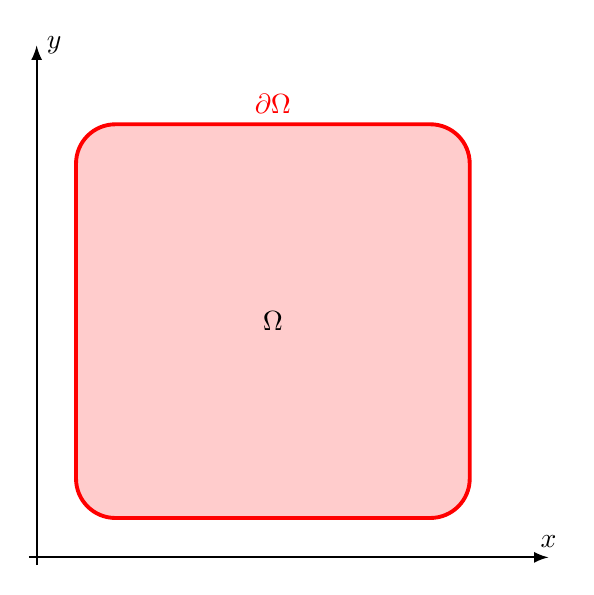
\begin{tikzpicture}[>=latex,thick]

\fill[color=red!20]
	(1,0.5)
	-- (5,0.5) to[out=0,in=-90] (5.5,1)
	-- (5.5,5) to[out=90,in=0] (5,5.5)
	-- (1,5.5) to[out=180,in=90] (0.5,5)
	-- (0.5,1) to[out=-90,in=180] (1,0.5) --cycle;

\draw[color=red,line width=1.4pt]
	(1,0.5)
	-- (5,0.5) to[out=0,in=-90] (5.5,1)
	-- (5.5,5) to[out=90,in=0] (5,5.5)
	-- (1,5.5) to[out=180,in=90] (0.5,5)
	-- (0.5,1) to[out=-90,in=180] (1,0.5) --cycle;

\node at (3,3) {$\Omega$};
\node[color=red] at (3,5.5) [above] {$\partial\Omega$};
	

\draw[->] (-0.1,0)--(6.5,0) coordinate[label={$x$}];
\draw[->] (0,-0.1)--(0,6.5) coordinate[label={right:$y$}];
\end{tikzpicture}
\end{center}
\end{column}
\end{columns}
\end{frame}
